\documentclass[twoside]{article}
\usepackage[utf8]{inputenc}
\usepackage[ngerman]{babel}
\usepackage{libertine}
\usepackage[a4paper]{geometry}
\usepackage{parskip}
\usepackage{amsmath, amsthm, amssymb, commath, mathtools}
\usepackage{physics}
\usepackage{nicefrac}
\usepackage{booktabs}
\usepackage{tabularx}
\usepackage{enumitem}
\usepackage{graphicx}
\usepackage{wrapfig}
\usepackage{caption}
\usepackage{float}
\usepackage{minted}
\usepackage{appendix}
\usepackage{icomma}
\usepackage{multirow}
\usepackage{multicol}
\usepackage{footmisc}
\usepackage[separate-uncertainty=true]{siunitx}
\sisetup{locale = DE}
\usepackage{xcolor}

\usepackage{csquotes}
\MakeOuterQuote{"}
\renewcommand{\ttdefault}{cmtt}

\usepackage{hyperref}
\usepackage{bookmark}
% https://tex.stackexchange.com/a/33701
\makeatletter
    \newcommand{\nonum}[0]{%
        \let\@oldseccntformat\@seccntformat %
        \renewcommand\@seccntformat[1]{}%
        }
    \newcommand{\resnum}[0]{\let\@seccntformat\@oldseccntformat}
\makeatother

\usepackage{chngcntr}
\counterwithin{figure}{section}

\newcommand{\versuch}[0]{ROT}
\newcommand{\versuchLang}[0]{Rotation}

\hypersetup{
	pdftitle={P1 -- \versuch{} Auswertung},
	pdfauthor={Yudong Sun},
	bookmarksnumbered=true,
	bookmarksopen=true,
	bookmarksopenlevel=2,
	pdfstartview=Fit,
	pdfpagemode=UseOutlines,
	colorlinks=true,
	linkcolor=black,
	filecolor=magenta,      
	urlcolor=blue
}
\urlstyle{same}

\title{\versuch -- \versuchLang \\ Auswertung}
\author{Yudong Sun \\{\small in Zusammenarbeit mit David Giesegh und Joel Schönberger}\\\\ Gruppe F2}

\usepackage{fancyhdr}
\pagestyle{fancy}
\fancyhf{}
\fancyhead[RO]{Yudong Sun}
\fancyhead[LO]{Auswertung -- \versuch}
\fancyhead[LE]{Yudong Sun}
\fancyhead[RE]{Auswertung -- \versuch}
\cfoot{\thepage}

% Custom Defs
\newcommand*{\ra}[1]{\renewcommand{\arraystretch}{#1}}
\newcommand*{\maxi}[1]{\text{max}\left(#1\right)}
\newcommand*{\mini}[1]{\text{min}\left(#1\right)}
\newcommand*{\todo}[1]{\textcolor{red}{TODO: #1}}
\newcommand*{\gnuplot}[0]{\texttt{gnuplot}}
\newcommand*{\sigfig}[1]{\hspace{0.5cm}\text{(#1 sig. Zif.)}}
\newcommand*{\overbar}[1]{\overline{\raisebox{0pt}[1.2\height]{$#1$}}} % https://tex.stackexchange.com/a/87615
% \addto\captionsngerman{
%     \let\oldfigname\figurename
%     \renewcommand{\figurename}{[\oldfigname}
%     \let\oldthefig\thefigure
%     \renewcommand{\thefigure}{\oldthefig]}
% } % https://tex.stackexchange.com/a/17490
% https://tex.stackexchange.com/a/101624 new line in caption

% Gaußsche Fehler Erzeuger
\makeatletter
    \newcommand{\gausserror}[2]{% \gausserror{G}{faktoren}
        \sqrt{%
            \@tempswafalse
            \@for\factor:=#2
            \do{
                \if@tempswa+%
                \else%
                    \@tempswatrue%
                \fi%
                \left(\pdv{#1}{\factor}\Delta\factor\right)^2%
            }%
        }
    }
\makeatother
% https://tex.stackexchange.com/a/59912
% https://riptutorial.com/latex/example/28657/loops---repeating-things

% / Custom Defs

\begin{document}

\maketitle

% Einstellungen
\nonum
\numberwithin{equation}{section}
% / Einstellungen

\section{Teilversuch 1: "Gewichtsverlust" des Maxwellschen Rads}
    Das Maxwellsche-Rad hat während des Auf- und Abrollens (außer Umkehrpunkt) immer eine nach unten gerichtete Beschleunigung. Diese Beschleunigung wirkt in derselben Richtung wie die Erdbeschleunigung. Im Vergleich zum Ruhezustand zieht das Maxwellsche-Rad deswegen nicht so viel auf dem Faden. Das folgt aus der sichtbaren Beschleunigung während des Auf- und Abrollens und dem Newtonsche 3. Gesetz. Die gemessene Kraft ist folglich geringer und die Waage hebt sich ab. 

    Am tiefsten Punkt kehrt das Rad um. Das führt zu einer Impulsänderung in einem kurzen Zeitintervall von einem maximalen Impuls nach unten zu einem maximalen Impuls nach oben. Mit $F = \dv{p}{t}$ versteht man diese Impulsänderung als eine große Kraft, die auf den Faden zieht. Diese Kraft wurde als einen Zuck auf der Waage beobachtet. 

    Die Gewichtskraft und die Seilkraft wirken immer auf dem Rad. Da das Rad ab und aufrollt, sind diese zwei Kräfte nicht im Gleichgewicht und es gibt eine resultierende externe Kraft, die den Translationsimpuls des Rads ändert. Da die Seilkraft nicht am Schwerpunkt des Rads greift, gibt es auch ein Drehmoment bezüglich der Rotationsachse des Rads, die den Drehimpuls ändert. 

    Es gibt deshalb zu jedem Zeitpunkt eine externe Kraft bzw. Drehmoment auf dem Rad, und folglich ist das Rad kein Inertialsystem. Die Translation- und Drehimpuls bleiben dann auch nicht konstant. 
\section{Teilversuch 2: Bestimmung eines Reflexiongrades}
	Mit $A =$ die korrigierte maximale Amplitude und $B =$ die korrigierte minimale Amplitude ist das Reflexionsgrad $R$ und folglich dessen Fehler laut der Anleitung gegeben durch:
	\begin{align}
		R &= \pbrace{\frac{A+B}{A-B}}^2 \label{eqn:tv2-1} \\
		\Delta R &= \gausserror{R}{A,B}
	\end{align}
	Die partielle Ableitungen liefern jeweils:
	\begin{align}
		\pdv{R}{A} &= 2 \pbrace{\frac{A-B}{A+B}}\sbrace{\frac{\cancel{A}+B-\pbrace{\cancel{A}-B}}{\pbrace{A+B}^2}} = 2 \pbrace{\frac{A-B}{A+B}} \sbrace{\frac{2B}{\pbrace{A+B}^2}} \notag \\
		&= 4\cdot \frac{B\pbrace{A-B}}{\pbrace{A+B}^3} \\
		\pdv{R}{B} &= 2 \pbrace{\frac{A-B}{A+B}}\sbrace{\frac{-\pbrace{A+\cancel{B}}-\pbrace{A-\cancel{B}}}{\pbrace{A+B}^2}} = 2 \pbrace{\frac{A-B}{A+B}} \sbrace{\frac{-2A}{\pbrace{A+B}^2}} \notag \\
		&= -4\cdot \frac{A\pbrace{A-B}}{\pbrace{A+B}^3}
	\end{align}
	Da $\Delta A = \Delta B = \sqrt{2}\cdot\Delta S$, lässt der Fehler wie folgt schreiben:
	\begin{equation}
		\Delta R = 4\sqrt{2}\Delta S \frac{A-B}{\pbrace{A+B}^3}\sqrt{A^2+B^2} \label{eqn:tv2-2}
	\end{equation}
	wobei $\Delta S =$ der Fehler bei jeder Messung der Mikrofonspannung.

	Die korrigierte Minima und Maxima werden hier als Zwischenergebnisse behandelt. Darum werden keine Fehler explizit berechnet. Die ist aber durch $\sqrt{2}\Delta S$ gegeben.

	Der Mittelwert $\overbar{R}$ und dessen Fehler $\Delta R$ mittels der Methode der oberen und unteren Grenzen sind dann:
	\begin{align}
		\overbar{R} &= \frac{\sum_{i=1}^3 R_i}{3} \label{eqn:tv2-3} \\
		\Delta \overbar{R} &= \frac{\sum_{i=1}^3 \pbrace{\cancel{R_i} + \Delta R_i} - \sum_{i=1}^3 \pbrace{\cancel{R_i} - \Delta R_i}}{3 \times 2}  = \frac{\sum_{i=1}^3 \Delta R_i + \cancel{\sum_{i=1}^3 \Delta R_i}}{3 \times \cancel{2}} \notag \\
		&= \frac{\sum_{i=1}^3 \Delta R_i}{3} \label{eqn:tv2-4}
	\end{align}
	Da es nur beim zweiten Teilaufgabe der Auswertung zum Teilversuch 2 gefragt, dass man der Fehler $\Delta \overbar{R}$ mittels der Methode der oberen und unteren Grenzen berechnen soll, ist die Korrektur für $A$ und $B$ mittels Gauß'sche Fehlerfortpflanzung gerechnet. Außerdem ist auch schwerig, schnell zu bestimmen, wann $A$ bzw. $B$ jeweils maximal und minimal sein, um das maximales und minimales $R$ zu bekommen. 

	Mit Gleichungen \eqref{eqn:tv2-1}, \eqref{eqn:tv2-2}, \eqref{eqn:tv2-3} und \eqref{eqn:tv2-4}, darstellen wir die Ergebnisse als Tabelle. Die Rechnungen erfolgt genauer in einem Tabellenkalkulationsprogramm. Die Werte hier sind schon gerundet. 
	\begin{center}
		\begin{tabular}{lrrr r}
			\toprule
			Paar $i$ & \num{1} & \num{2} & \num{3} & \\
			\midrule
			Min $S_\text{min} / \si{\milli\volt}$ & \num{5.8} & \num{6.2} & \num{6.0} & \\
			Hintergr. $S_\text{min HG} / \si{\milli\volt}$ & \num{0.9} & \num{0.9} & \num{0.9} & \\
			Max $S_\text{max} / \si{\milli\volt}$ &\num{20.7} & \num{20.1} & \num{20.5} & \\
			Hintergr. $S_\text{max HG} / \si{\milli\volt}$ & \num{0.9} & \num{0.9} & \num{1.0} & \\
			\midrule
			$B / \si{\milli\volt}$ & \num{4.9} & \num{5.3} & \num{5.1} & \\
			$A / \si{\milli\volt}$ & \num{19.8} & \num{19.2} & \num{19.5} & \\
			$R$ & \num{0.364} & \num{0.322} & \num{0.343} & $\overbar{R} = \num{0.343}$ \\
			$\Delta R$ & \num{0.023} & \num{0.022} & \num{0.023} & $\Delta \overbar{R} = \num{0.023}$ \\
			\bottomrule
		\end{tabular}
	\end{center}
	Explizit geschrieben: $R = \num{0.343(23)}$. $R$ is einheitslos. 

	Als Funktion der Energie ist $R$ gegeben durch:
	\begin{equation}
		R = \frac{b^2}{a^2} = \frac{\text{Energie der reflektierten Welle}}{\text{Energie der Quellwelle}}
	\end{equation}
	Laut Energieerhaltungssatz kann die reflektierte Welle keine Energie mehr als die Quellwelle haben. Das heißt, dass $b < a$ bzw. $R \in \sbrace{0,1}$ sein muss. In diesem Fall liegt unser Wert von $R$ in diesem Intervall, was physikalischen Sinn ergibt.

	In unserem Versuch ist $\SI{34.3(23)}{\percent}$ der Energieflussdichte am offenen Rohrende reflektiert und $\SI{100}{\percent} - \SI{34.3(23)}{\percent} = \SI{65.7(23)}{\percent}$ transmittiert.   
\newpage
\section{Teilversuch 3: Messung der Eigenfrequenzen einer Luftsäule}
	Fehler bei Messung bzw. Steuerung der Frequenz $\Delta f_n = \SI{1}{\hertz}$\\
	Fehler bei Messung der Mikrofonspannung $\Delta U_\text{eff} = \SI{0.1}{\milli\volt}$

	\begin{center}
		\begin{tabular}{l *{11}{r}}
			\toprule
			$n$ & \num{0} & \num{1} & \num{2} & \num{3} & \num{4} & \num{5} & \num{6} & \num{7} & \num{8} & \num{9} & \num{10} \\
			\midrule
			$f_n / \si{\hertz}$ & \num{168} & \num{502} & \num{837} & \num{1171} & \num{1510} & \num{1843} & \num{2188} & \num{2541} & \num{2876} & \num{3210} & \num{3554} \\
			$U_\text{eff} / \si{\milli\volt}$ & \num{3.36} & \num{22.10} & \num{57.7} & \num{31.07} & \num{21.70} & \num{22.48} & \num{22.93} & \num{24.80} & \num{13.20} & \num{10.10} & \num{6.76} \\
			\bottomrule
		\end{tabular}
	\end{center}
	Laut Gleichung (6) der Anleitung hat $f_n$ und $n$ den folgenden Zusammenhang:
	\begin{equation}
		f_n = \frac{v}{4L^{*}} \pbrace{2n +1} = \left(\frac{v}{2L^{*}}\right)n + \frac{v}{4L^{*}} \equiv an+b
	\end{equation}
	Daraus folgt auch, dass die akustische Rohrlänge $L^{*}$ und der dazugehörige Fehler $\Delta L^{*}$ sich wie folgt brechnen lässt:
	\begin{align}
		L^{*} &= \frac{v}{2a} \label{eqn:akustiklange}\\
		\Delta L^{*} &= \gausserror{L^{*}}{v,a} \overset{\text{\scriptsize (AMW)}}{=} \frac{v}{2a}\sqrt{\pbrace{\frac{\Delta v}{v}}^2 + \pbrace{\frac{\Delta a}{a}}^2} \label{eqn:deltaakustiklange}
	\end{align}

	Die Daten wurden mit \gnuplot{} geplottet und eine Kurveanpassung wurde durchgeführt (Siehe Appendix \ref{appdx:gnuplotTV3}).
	\begin{figure}[H]
		\centering
		% GNUPLOT: LaTeX picture with Postscript
\begingroup
  \makeatletter
  \providecommand\color[2][]{%
    \GenericError{(gnuplot) \space\space\space\@spaces}{%
      Package color not loaded in conjunction with
      terminal option `colourtext'%
    }{See the gnuplot documentation for explanation.%
    }{Either use 'blacktext' in gnuplot or load the package
      color.sty in LaTeX.}%
    \renewcommand\color[2][]{}%
  }%
  \providecommand\includegraphics[2][]{%
    \GenericError{(gnuplot) \space\space\space\@spaces}{%
      Package graphicx or graphics not loaded%
    }{See the gnuplot documentation for explanation.%
    }{The gnuplot epslatex terminal needs graphicx.sty or graphics.sty.}%
    \renewcommand\includegraphics[2][]{}%
  }%
  \providecommand\rotatebox[2]{#2}%
  \@ifundefined{ifGPcolor}{%
    \newif\ifGPcolor
    \GPcolortrue
  }{}%
  \@ifundefined{ifGPblacktext}{%
    \newif\ifGPblacktext
    \GPblacktexttrue
  }{}%
  % define a \g@addto@macro without @ in the name:
  \let\gplgaddtomacro\g@addto@macro
  % define empty templates for all commands taking text:
  \gdef\gplbacktext{}%
  \gdef\gplfronttext{}%
  \makeatother
  \ifGPblacktext
    % no textcolor at all
    \def\colorrgb#1{}%
    \def\colorgray#1{}%
  \else
    % gray or color?
    \ifGPcolor
      \def\colorrgb#1{\color[rgb]{#1}}%
      \def\colorgray#1{\color[gray]{#1}}%
      \expandafter\def\csname LTw\endcsname{\color{white}}%
      \expandafter\def\csname LTb\endcsname{\color{black}}%
      \expandafter\def\csname LTa\endcsname{\color{black}}%
      \expandafter\def\csname LT0\endcsname{\color[rgb]{1,0,0}}%
      \expandafter\def\csname LT1\endcsname{\color[rgb]{0,1,0}}%
      \expandafter\def\csname LT2\endcsname{\color[rgb]{0,0,1}}%
      \expandafter\def\csname LT3\endcsname{\color[rgb]{1,0,1}}%
      \expandafter\def\csname LT4\endcsname{\color[rgb]{0,1,1}}%
      \expandafter\def\csname LT5\endcsname{\color[rgb]{1,1,0}}%
      \expandafter\def\csname LT6\endcsname{\color[rgb]{0,0,0}}%
      \expandafter\def\csname LT7\endcsname{\color[rgb]{1,0.3,0}}%
      \expandafter\def\csname LT8\endcsname{\color[rgb]{0.5,0.5,0.5}}%
    \else
      % gray
      \def\colorrgb#1{\color{black}}%
      \def\colorgray#1{\color[gray]{#1}}%
      \expandafter\def\csname LTw\endcsname{\color{white}}%
      \expandafter\def\csname LTb\endcsname{\color{black}}%
      \expandafter\def\csname LTa\endcsname{\color{black}}%
      \expandafter\def\csname LT0\endcsname{\color{black}}%
      \expandafter\def\csname LT1\endcsname{\color{black}}%
      \expandafter\def\csname LT2\endcsname{\color{black}}%
      \expandafter\def\csname LT3\endcsname{\color{black}}%
      \expandafter\def\csname LT4\endcsname{\color{black}}%
      \expandafter\def\csname LT5\endcsname{\color{black}}%
      \expandafter\def\csname LT6\endcsname{\color{black}}%
      \expandafter\def\csname LT7\endcsname{\color{black}}%
      \expandafter\def\csname LT8\endcsname{\color{black}}%
    \fi
  \fi
    \setlength{\unitlength}{0.0500bp}%
    \ifx\gptboxheight\undefined%
      \newlength{\gptboxheight}%
      \newlength{\gptboxwidth}%
      \newsavebox{\gptboxtext}%
    \fi%
    \setlength{\fboxrule}{0.5pt}%
    \setlength{\fboxsep}{1pt}%
\begin{picture}(7200.00,5040.00)%
    \gplgaddtomacro\gplbacktext{%
      \csname LTb\endcsname%%
      \put(814,704){\makebox(0,0)[r]{\strut{}$4,2$}}%
      \put(814,1112){\makebox(0,0)[r]{\strut{}$4,4$}}%
      \put(814,1521){\makebox(0,0)[r]{\strut{}$4,6$}}%
      \put(814,1929){\makebox(0,0)[r]{\strut{}$4,8$}}%
      \put(814,2337){\makebox(0,0)[r]{\strut{}$5$}}%
      \put(814,2746){\makebox(0,0)[r]{\strut{}$5,2$}}%
      \put(814,3154){\makebox(0,0)[r]{\strut{}$5,4$}}%
      \put(814,3562){\makebox(0,0)[r]{\strut{}$5,6$}}%
      \put(814,3971){\makebox(0,0)[r]{\strut{}$5,8$}}%
      \put(814,4379){\makebox(0,0)[r]{\strut{}$6$}}%
      \put(946,484){\makebox(0,0){\strut{}$-100$}}%
      \put(1478,484){\makebox(0,0){\strut{}$0$}}%
      \put(2011,484){\makebox(0,0){\strut{}$100$}}%
      \put(2543,484){\makebox(0,0){\strut{}$200$}}%
      \put(3076,484){\makebox(0,0){\strut{}$300$}}%
      \put(3608,484){\makebox(0,0){\strut{}$400$}}%
      \put(4141,484){\makebox(0,0){\strut{}$500$}}%
      \put(4673,484){\makebox(0,0){\strut{}$600$}}%
      \put(5206,484){\makebox(0,0){\strut{}$700$}}%
      \put(5738,484){\makebox(0,0){\strut{}$800$}}%
      \put(6271,484){\makebox(0,0){\strut{}$900$}}%
      \put(6803,484){\makebox(0,0){\strut{}$1000$}}%
    }%
    \gplgaddtomacro\gplfronttext{%
      \csname LTb\endcsname%%
      \put(209,2541){\rotatebox{-270}{\makebox(0,0){\strut{}$\ln \left[\left(h - h_\infty\right) / \si{\milli\meter}\right]$}}}%
      \put(3874,154){\makebox(0,0){\strut{}Zeit $t$ ($\si{\second}$)}}%
      \put(3874,4709){\makebox(0,0){\strut{}Wasserstand beim Kapilarviskosimeter im Verlauf der Zeit}}%
      \csname LTb\endcsname%%
      \put(5816,4206){\makebox(0,0)[r]{\strut{}$-0,00158x + 5,80951$}}%
      \csname LTb\endcsname%%
      \put(5816,3986){\makebox(0,0)[r]{\strut{}tv3.dat}}%
    }%
    \gplbacktext
    \put(0,0){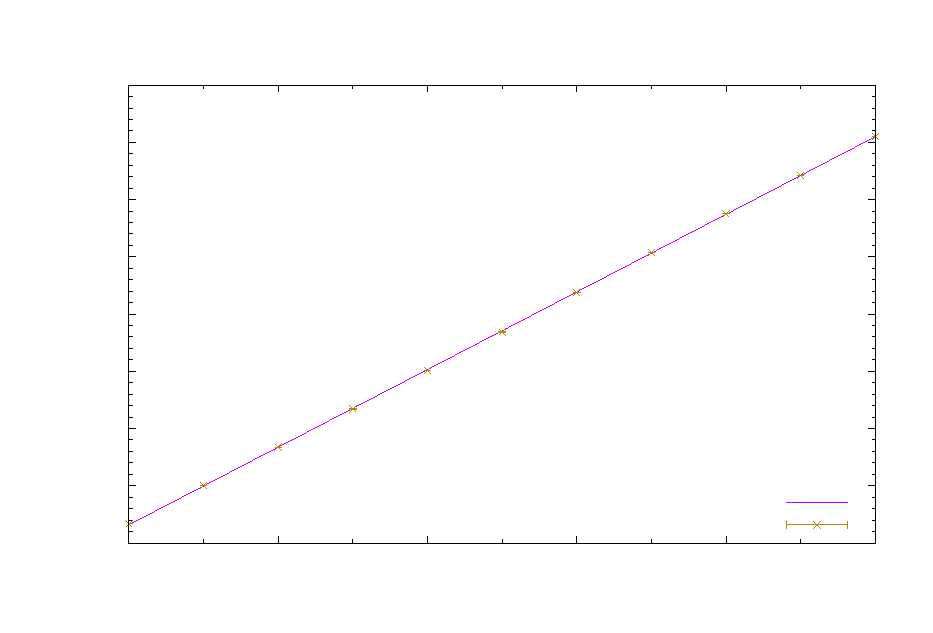
\includegraphics{tv3-plot}}%
    \gplfronttext
  \end{picture}%
\endgroup

		\caption{\centering Messung der Oberschwingungen des Rohres\captionbr $\chi^2_{\text{red}} = \num{46.698} > 1 \implies$ Schlechte Anpassung}
		\label{fig:tvthree-plot}
		\vspace{-1em}
	\end{figure}
	Die schlechte Anpassung kann vermutlich dadurch erklärt werden, dass die Bestimmung der Resonanzfrequenzen eher ungenau war, besonders bei der Steuerung des Sinus-Generator. In diesem Fall wurden aber die Messungenauigkeit der Frequenzen schon bei der Kurvenanpassung berücksichtigt. Es könnte dann sein, dass wir diese Ungenauigkeit wesentlich unterschätzt haben. 

	Als Endergebnis erhalten wir:
	\begin{center}
		\begin{tabular}{l r r}
			\toprule
			Variable & Rohausgabe & Gerundet \\
			\midrule
			$a$ & \SI{339,0636(6516)}{\hertz} & \SI{339.1(7)}{\hertz} \\
			$b$ & \SI{159.227(3855)}{\hertz} & \SI{159(4)}{\hertz} \\
			\bottomrule
		\end{tabular}
	\end{center}
	Wir benutzen in unserer Rechnungen die genauere Werte von $a$ und $\Delta a$ bzw. $v$ und $\Delta v$. In diesem Fall wurde für die Bestimmung der akustischen Rohrlänge aufgrund des geringeren Fehler $a$ statt $b$ gewählt, obwohl beide Werte theoretisch funktionieren könnten. 

	Mit der folgenden Werten:
    \begin{center}
        \begin{tabular}{lrl}
            \toprule
            Variable & Wert & Bedeutung \\
            \midrule
            $a$ & \SI{339,0636(6516)}{\hertz} & Gefundene Steigung der Gerade \\
            $v$ & \SI{344,424(1694)}{\meter\per\second} & Gefundene Schallgeschwindigkeit \\
            \bottomrule
        \end{tabular}
    \end{center}
    lässt sich mittels Gleichungen \eqref{eqn:akustiklange} und \eqref{eqn:deltaakustiklange} die akustische Rohrlänge $L^{*}$ und deren Fehler $\Delta L^{*}$ bestimmen:
    \begin{align}
    	L^{*} &= \frac{\SI{344,424}{\meter\per\second}}{2\pbrace{\SI{339,0636}{\hertz}}} = \SI{0,507905}{\meter} \sigfig{6} \\
    	\Delta L^{*} &= \frac{\SI{344,424}{\meter\per\second}}{2\pbrace{\SI{339,0636}{\hertz}}} \sqrt{\pbrace{\frac{\SI{1.694}{\meter\per\second}}{\SI{344,424}{\meter\per\second}}}^2 + \pbrace{\frac{\SI{0.6516}{\hertz}}{\SI{339,0636}{\hertz}}}^2} \notag \\
    	&= \SI{2,682e-3}{\meter} \sigfig{4}
    \end{align}
    Daraus folgt, dass die akustische Rohrlänge $L^{*} = \SI{0,5079(27)}{\meter} = \SI{507.9(27)}{\milli\meter}$.

    Im Vergleich dazu ist die gemessene Rohrlänge $L = \SI{50.0(1)}{\centi\meter} = \SI{500(1)}{\milli\meter}$. Das Fehlerintervall der beiden Werten überschneiden sich miteinander nicht, also ist $L^{*} > L$, was zu erwarten ist. 
\newpage
\section{Teilversuch 4: Messung der Resonanzkurve für eine Oberschwingung}
	\subsection{Messreihe}
	Fehler der Frequenzen $\Delta f = \SI{1}{\hertz}$ \\
	Fehler der Spannung $\Delta f = \SI{0.2}{\milli\volt}$

	Raumhintergrund $= \SI{1.1(2)}{\milli\volt}$

	\begin{center}
		\begin{tabular}{l *{10}{r}}
			\toprule
			$f / \si{\hertz}$ & \num{1011} & \num{980} & \num{970} & \num{952} & \num{928} & \num{910} & \num{892} & \num{881} & \num{871} & \num{861} \\
			\midrule
			$U_\text{eff} / \si{\milli\volt}$ & \num{7.33} & \num{7.53} & \num{7.99} & \num{8.85} & \num{10.85} & \num{13.45} & \num{18.33} & \num{23.31} & \num{30.14} & \num{44.53} \\
			\bottomrule
			\toprule
			$f / \si{\hertz}$ & \num{854} & \num{850} & \num{844} & \num{841} & \num{837} & \num{833} & \num{830} & \num{825} & \num{818} & \num{810} \\
			\midrule
			$U_\text{eff} / \si{\milli\volt}$ & \num{64.33} & \num{85.80} & \num{125.53} & \num{149.11} & \num{149.49} & \num{120.65} & \num{96.04} & \num{71.73} & \num{54.43} & \num{41.24} \\
			\bottomrule
			\toprule
			$f / \si{\hertz}$ & \num{801} & \num{790} & \num{780} & \num{760} & \num{742}  \\
			\midrule
			$U_\text{eff} / \si{\milli\volt}$ & \num{34.00} & \num{28.51} & \num{25.66} & \num{22.68} & \num{21.61} \\
			\bottomrule
		\end{tabular}
	\end{center}

	\subsection{Graph}
	Aus der Anleitung des Versuchs MOS lässt die folgende Funktion eine Resonanzkurve beschreiben:
	\begin{equation}
		\hat{x} = \frac{\omega_0^2}{\sqrt{\pbrace{\omega_0^2 - \omega^2}^2+\pbrace{2\beta\omega}^2}}~\hat{x}_\text{A} \iff U_\text{eff} = \frac{f_0^2}{\sqrt{\pbrace{f_0^2 - f^2}^2+\pbrace{2\beta f}^2}}~U_\text{A}
	\end{equation}

	Da die Kurvenanpassung mit \gnuplot{} sehr empfindlich auf die Wahl der Startparameter reagiert, müssen die Startparameter sorgfältig ausgewählt. Dafür ist eine grobe Kurveanpassung wie im Versuch MOS mittels Geogebra per Hand durchgeführt:
	\begin{figure}[H]
		\centering
		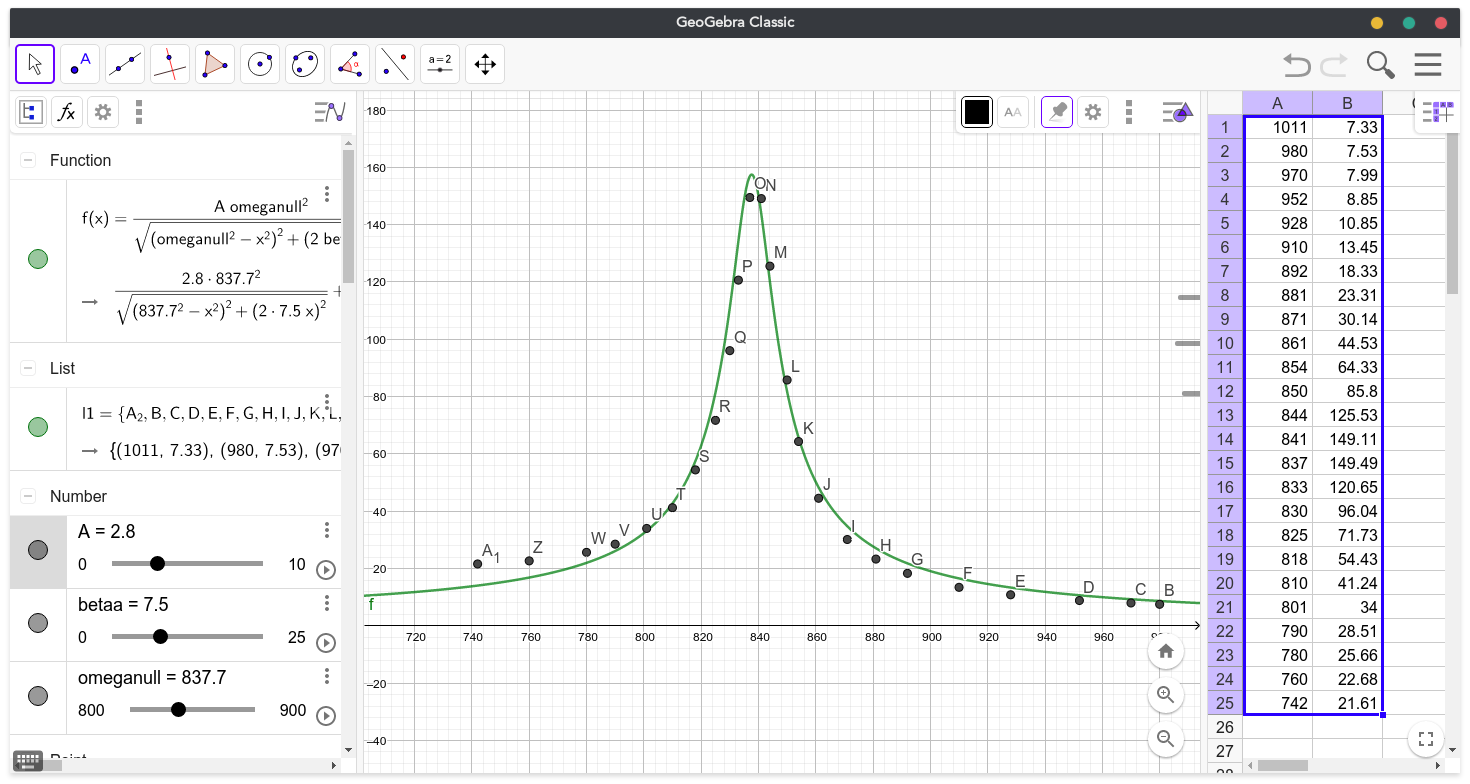
\includegraphics[width=0.9\textwidth]{geogebra.png}
		\caption{Grobe Kurveanpassung mittels Geogebra}
	\end{figure}

	Der Raumhintergrund und dessen Fehler sind direkt im \gnuplot{} Skript berücksichtigt (Siehe Appendix \ref{appdx:gnuplotTV4}). Der Fehler der Spannung nach dem Abzug des Raumhintergrund wird als $(\SI{0.2}{\milli\volt} + \SI{0.2}{\milli\volt} = \SI{0.4}{\milli\volt})$ angenommen. Der Grund dafür ist, dass wir letztendlich nur eine Messung von der Raumhintergrund haben, obwohl wir bei mehrfache Messungen eher Schwankungen gegen die gleiche Werten bekommen. Daher ist es sicherer bei der Kurvenanpassung einen größeren Fehler zu benutzen.

	\begin{figure}[H]
		\centering
		% GNUPLOT: LaTeX picture with Postscript
\begingroup
  \makeatletter
  \providecommand\color[2][]{%
    \GenericError{(gnuplot) \space\space\space\@spaces}{%
      Package color not loaded in conjunction with
      terminal option `colourtext'%
    }{See the gnuplot documentation for explanation.%
    }{Either use 'blacktext' in gnuplot or load the package
      color.sty in LaTeX.}%
    \renewcommand\color[2][]{}%
  }%
  \providecommand\includegraphics[2][]{%
    \GenericError{(gnuplot) \space\space\space\@spaces}{%
      Package graphicx or graphics not loaded%
    }{See the gnuplot documentation for explanation.%
    }{The gnuplot epslatex terminal needs graphicx.sty or graphics.sty.}%
    \renewcommand\includegraphics[2][]{}%
  }%
  \providecommand\rotatebox[2]{#2}%
  \@ifundefined{ifGPcolor}{%
    \newif\ifGPcolor
    \GPcolortrue
  }{}%
  \@ifundefined{ifGPblacktext}{%
    \newif\ifGPblacktext
    \GPblacktexttrue
  }{}%
  % define a \g@addto@macro without @ in the name:
  \let\gplgaddtomacro\g@addto@macro
  % define empty templates for all commands taking text:
  \gdef\gplbacktext{}%
  \gdef\gplfronttext{}%
  \makeatother
  \ifGPblacktext
    % no textcolor at all
    \def\colorrgb#1{}%
    \def\colorgray#1{}%
  \else
    % gray or color?
    \ifGPcolor
      \def\colorrgb#1{\color[rgb]{#1}}%
      \def\colorgray#1{\color[gray]{#1}}%
      \expandafter\def\csname LTw\endcsname{\color{white}}%
      \expandafter\def\csname LTb\endcsname{\color{black}}%
      \expandafter\def\csname LTa\endcsname{\color{black}}%
      \expandafter\def\csname LT0\endcsname{\color[rgb]{1,0,0}}%
      \expandafter\def\csname LT1\endcsname{\color[rgb]{0,1,0}}%
      \expandafter\def\csname LT2\endcsname{\color[rgb]{0,0,1}}%
      \expandafter\def\csname LT3\endcsname{\color[rgb]{1,0,1}}%
      \expandafter\def\csname LT4\endcsname{\color[rgb]{0,1,1}}%
      \expandafter\def\csname LT5\endcsname{\color[rgb]{1,1,0}}%
      \expandafter\def\csname LT6\endcsname{\color[rgb]{0,0,0}}%
      \expandafter\def\csname LT7\endcsname{\color[rgb]{1,0.3,0}}%
      \expandafter\def\csname LT8\endcsname{\color[rgb]{0.5,0.5,0.5}}%
    \else
      % gray
      \def\colorrgb#1{\color{black}}%
      \def\colorgray#1{\color[gray]{#1}}%
      \expandafter\def\csname LTw\endcsname{\color{white}}%
      \expandafter\def\csname LTb\endcsname{\color{black}}%
      \expandafter\def\csname LTa\endcsname{\color{black}}%
      \expandafter\def\csname LT0\endcsname{\color{black}}%
      \expandafter\def\csname LT1\endcsname{\color{black}}%
      \expandafter\def\csname LT2\endcsname{\color{black}}%
      \expandafter\def\csname LT3\endcsname{\color{black}}%
      \expandafter\def\csname LT4\endcsname{\color{black}}%
      \expandafter\def\csname LT5\endcsname{\color{black}}%
      \expandafter\def\csname LT6\endcsname{\color{black}}%
      \expandafter\def\csname LT7\endcsname{\color{black}}%
      \expandafter\def\csname LT8\endcsname{\color{black}}%
    \fi
  \fi
    \setlength{\unitlength}{0.0500bp}%
    \ifx\gptboxheight\undefined%
      \newlength{\gptboxheight}%
      \newlength{\gptboxwidth}%
      \newsavebox{\gptboxtext}%
    \fi%
    \setlength{\fboxrule}{0.5pt}%
    \setlength{\fboxsep}{1pt}%
\begin{picture}(8640.00,5760.00)%
    \gplgaddtomacro\gplbacktext{%
      \csname LTb\endcsname%%
      \put(814,704){\makebox(0,0)[r]{\strut{}$0$}}%
      \put(814,1253){\makebox(0,0)[r]{\strut{}$20$}}%
      \put(814,1803){\makebox(0,0)[r]{\strut{}$40$}}%
      \put(814,2352){\makebox(0,0)[r]{\strut{}$60$}}%
      \put(814,2902){\makebox(0,0)[r]{\strut{}$80$}}%
      \put(814,3451){\makebox(0,0)[r]{\strut{}$100$}}%
      \put(814,4000){\makebox(0,0)[r]{\strut{}$120$}}%
      \put(814,4550){\makebox(0,0)[r]{\strut{}$140$}}%
      \put(814,5099){\makebox(0,0)[r]{\strut{}$160$}}%
      \put(946,484){\makebox(0,0){\strut{}$700$}}%
      \put(1988,484){\makebox(0,0){\strut{}$750$}}%
      \put(3031,484){\makebox(0,0){\strut{}$800$}}%
      \put(4073,484){\makebox(0,0){\strut{}$850$}}%
      \put(5116,484){\makebox(0,0){\strut{}$900$}}%
      \put(6158,484){\makebox(0,0){\strut{}$950$}}%
      \put(7201,484){\makebox(0,0){\strut{}$1000$}}%
      \put(8243,484){\makebox(0,0){\strut{}$1050$}}%
    }%
    \gplgaddtomacro\gplfronttext{%
      \csname LTb\endcsname%%
      \put(209,2901){\rotatebox{-270}{\makebox(0,0){\strut{}Mikrofonspannung $U_\text{eff}$ ($\si{\milli\volt}$)}}}%
      \put(4594,154){\makebox(0,0){\strut{}Frequenz $f$ ($\si{\hertz}$)}}%
      \put(4594,5429){\makebox(0,0){\strut{}Resonanzkurve des Rohres bei der 2. Oberschwingung}}%
      \csname LTb\endcsname%%
      \put(7256,4926){\makebox(0,0)[r]{\strut{}Angepasste Kurve}}%
      \csname LTb\endcsname%%
      \put(7256,4706){\makebox(0,0)[r]{\strut{}Messpunkte}}%
    }%
    \gplbacktext
    \put(0,0){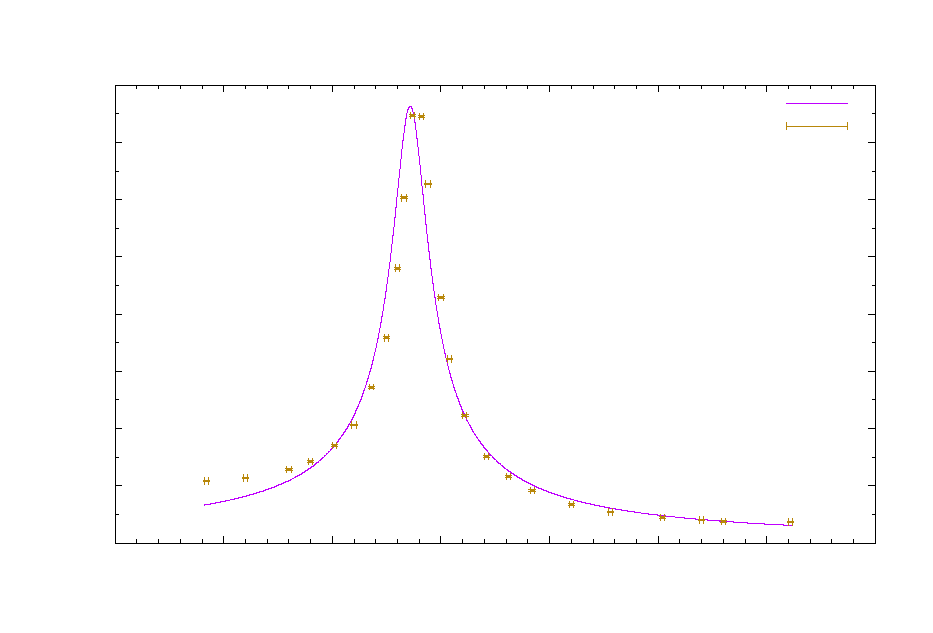
\includegraphics{tv4-plot}}%
    \gplfronttext
  \end{picture}%
\endgroup

		\caption{\centering Messung der Resonanzkurve des Rohres bei der 2. Oberschwingung\captionbr $\chi^2_{\text{red}} = \num{32.6373} > 1 \implies$ Schlechte Anpassung}
		\label{fig:tvfour-plot}
		\vspace{-1em}
	\end{figure}
	Als Endergebnis erhalten wir:
	\begin{center}
		\begin{tabular}{l r r}
			\toprule
			Variable & Rohausgabe & Gerundet \\
			\midrule
			$f_0$ & \SI{835.89(146)}{\hertz} & \SI{835.9(15)}{\hertz} \\
			$U_\text{A}$ & \SI{2.8473(1317)}{\milli\volt} & \SI{2.85(14)}{\milli\volt} \\
			$\beta$ & \num{7.79(102)} & \num{7.8(11)} \\
			\bottomrule
		\end{tabular}
	\end{center}

	Anstatt einfach die Messpunkte durch eine glatte Kurve zu verbinden, war eine theoretische Kurve auf die Messwerte angepasst. Die Anpassung war leider schlecht, und der Grund dafür liegt vermütlich daran, dass wir Nebeneffekte bzw. andere Faktoren nicht berücksichtigt haben. Es könnte auch sein, dass wir alle Werten im SI Einheiten skalieren sollten, bevor wir die Kurvenanpassung durchführen. 

	Unsere gemessene Resonanzfrequenz $f_0 = \SI{837(1)}{\hertz}$ liegt auch im Fehlerintervall des aus der Kurvenanpassung gefundene $f_0$. Die Werte stimmen also miteinander überein.
\setcounter{section}{4}
\section{Teilversuch 5: Sinken von Kugeln in einer viskosen Flüssigkeit}
	\subsection{Verhältnis aus Rohrradius $R$ und Kugelradius $r$}
		\subsubsection{Kugel}
			Fehler bei Messung des Kugeldurchmessers $= \SI{0.01}{\milli\meter}$

			\begin{center}
				\begin{tabular}{l r r r}
					\toprule
					Messung $n$ & $1$ & $2$ & $\overbar{d_i}$\\
					\midrule
					Durchmesser der kleinen Kugel $d_k$ / \si{\milli\meter} & \num{0.98} & \num{0.99} & \num{0.985}\\
					Durchmesser der großen Kugel $d_g$ / \si{\milli\meter} & \num{2.99} & \num{2.99} & \num{2.990} \\
					\bottomrule
				\end{tabular}
			\end{center}
			Der Mittelwerte $\overbar{d_i}$, $i = g, k$ wurden wie folgt berechnet:
	        \begin{equation}
	            \Delta d \coloneqq \overbar{d_i} = \frac{1}{N} \left(\sum_{x=1}^{N} d_{in} \right) = \frac{1}{2} \left(\sum_{x=1}^{2} d_{in} \right) \label{eqn:mittelwert}
	        \end{equation}
	        \newpage
	        Da alle Messungen stochastisch unabhängig sind, benutzen wir hier die Gauß'scher Fehlerfortpflanzung:
	        \begin{equation}
	            \Delta \overbar{d_i} = \frac{\Delta d_i}{\sqrt{N}} = \frac{\Delta d_i}{\sqrt{2}} = \frac{\SI{0.01}{\milli\meter}}{\sqrt{2}} = \SI{0.008}{\milli\meter} \label{eqn:mittelfehler}
	        \end{equation}

	    \subsubsection{Rohr}
		    \begin{center}
		    	\begin{tabular}{l r}
		    		Innendurchmesser des kleinen Rohres $D_k$ & \SI{9.95(5)}{\milli\meter} \\
		    		Innendurchmesser des großen Rohres $D_g$  & \SI{55.45(5)}{\milli\meter} \\
		    	\end{tabular}
		    \end{center}

		\subsubsection{Verhältnisse}
			Die Verhältnis $k$ aus Rohrradius $R$ und $r$ und der dazugehörige Fehler $\Delta k$ sind gegeben durch:
			\begin{align}
				k &= \frac{R}{r} = \frac{D}{d} \\
				\Delta k &= \gausserror{k}{D,d} = \sqrt{\pbrace{\frac{\Delta D}{d}}^2 + \pbrace{\frac{D}{d^2} \Delta d}^2} \notag \\
				&= \frac{1}{d}\sqrt{\pbrace{\Delta D}^2 + \pbrace{\frac{D}{d} \Delta d}^2} \label{eqn:kfehler}
			\end{align}
			$k$ ist Einheitslos.

			\iu{Kleine Kugel, Kleines Rohr}
			\begin{align}
				k &= \frac{D_k}{d_k} = \frac{\SI{9.95}{\milli\meter}}{\SI{0.985}{\milli\meter}} = \num{10.1015} \sigfig{6} \\
				\Delta k &= \frac{1}{\SI{0.985}{\milli\meter}}\sqrt{\pbrace{\SI{0.05}{\milli\meter}}^2 + \pbrace{\frac{\SI{9.95}{\milli\meter}}{\SI{0.985}{\milli\meter}} \pbrace{\frac{\SI{0.01}{\milli\meter}}{\sqrt{2}}}}^2} \notag \\
				&= \num{0.0886} \sigfig{3} \\
				\implies &k_{kK} = \num{10.10(9)}
			\end{align}

			\iu{Kleine Kugel, Großes Rohr}
			\begin{align}
				k &= \frac{D_g}{d_k} = \frac{\SI{55.45}{\milli\meter}}{\SI{0.985}{\milli\meter}} = \num{56,2944} \sigfig{6} \\
				\Delta k &= \frac{1}{\SI{0.985}{\milli\meter}}\sqrt{\pbrace{\SI{0.05}{\milli\meter}}^2 + \pbrace{\frac{\SI{55.45}{\milli\meter}}{\SI{0.985}{\milli\meter}} \pbrace{\frac{\SI{0.01}{\milli\meter}}{\sqrt{2}}}}^2} \notag \\
				&= \num{0,408} \sigfig{3} \\
				\implies &k_{kG} = \num{56,3(5)}
			\end{align}

			\iu{Große Kugel, Kleines Rohr}
			\begin{align}
				k &= \frac{D_k}{d_g} = \frac{\SI{9.95}{\milli\meter}}{\SI{2,990}{\milli\meter}} = \num{3.32776} \sigfig{6} \\
				\Delta k &= \frac{1}{\SI{2,990}{\milli\meter}}\sqrt{\pbrace{\SI{0.05}{\milli\meter}}^2 + \pbrace{\frac{\SI{9.95}{\milli\meter}}{\SI{2,990}{\milli\meter}} \pbrace{\frac{\SI{0.01}{\milli\meter}}{\sqrt{2}}}}^2} \notag \\
				&= \num{0.0185} \sigfig{3} \\
				\implies &k_{gK} = \num{3.328(19)}
			\end{align}

			\iu{Große Kugel, Großes Rohr}
			\begin{align}
				k &= \frac{D_g}{d_k} = \frac{\SI{55.45}{\milli\meter}}{\SI{2,990}{\milli\meter}} = \num{18.5452} \sigfig{6} \\
				\Delta k &= \frac{1}{\SI{2,990}{\milli\meter}}\sqrt{\pbrace{\SI{0.05}{\milli\meter}}^2 + \pbrace{\frac{\SI{55.45}{\milli\meter}}{\SI{2,990}{\milli\meter}} \pbrace{\frac{\SI{0.01}{\milli\meter}}{\sqrt{2}}}}^2} \notag \\
				&= \num{0.0470} \sigfig{3} \\
				\implies &k_{gG} = \num{18.55(5)}
			\end{align}

			Tabuliert haben wir für $k$:
			\begin{center}
				\begin{tabular}{l | r r}
				& Kleine Kugel & Große Kugel \\
				\midrule
				Kleines Rohr & \num{10.10(9)} & \num{3.328(19)} \\ 
				Großes Rohr & \num{56,3(5)} & \num{18.55(5)}
				\end{tabular}
			\end{center}
	\newpage
	\subsection{Sinkgeschwindigkeiten}
		Angenommen, dass die Kugeln eine konstante Geschwindigkeit während des Sinkens haben, dann lässt sich die Sinkgeschwindigkeit $v$ und der dazugehörige Fehler $\Delta k$ durch einfache Kinematik bestimmen:
		\begin{align}
			v &= \frac{s}{t} \\
			\Delta v &\overset{\eqref{eqn:kfehler}}{=} \frac{1}{t}\times\sqrt{\pbrace{\Delta s}^2 + \pbrace{\frac{s}{t} \Delta t}^2}
		\end{align}
		wobei $s =$ Höhe der Fallstrecke und $t =$ Fallzeit.

		Als Fallstrecke haben wir immer $s = \SI{801(1)}{\milli\meter}$.

		Für die Fallzeiten haben wir immer einen Fehler von $\SI{0.2}{\second}$.

		\iu{Kleine Kugel, Weites Rohr}

		Als Fallzeiten der kleine Kugel im weiten Rohr haben wir:
		\begin{center}
			\begin{tabular}{l rrr r}
				\toprule
				Messung & \num{1} & \num{2} & \num{3} & $\overbar{t_i}$ \\ 
				\midrule
				Fallzeit $t_i$ / \si{\second} & \num{109.02} & \num{109.09} & \num{109.30} & \num{109.137} \\
				\bottomrule
			\end{tabular}
		\end{center}
		Die Rechnung für den Mittelwert erfolgt wie bei Gleichung \eqref{eqn:mittelwert} mit $N = 3$. Der Fehler ist dann analog zu \eqref{eqn:mittelfehler} $= \SI{0.2}{\second} / \sqrt{3} = \SI{0.12}{\second}$.

		$v$ und $\Delta v$ sind dann gegeben durch:
		\begin{align}
			v &= \frac{\SI{801}{\milli\meter}}{\SI{109.137}{\second}} = \SI{7.33942}{\milli\meter\per\second} \sigfig{6} \\
			\Delta v &= \frac{1}{\SI{109.137}{\second}}\times\sqrt{\pbrace{\SI{1}{\milli\meter}}^2 + \pbrace{\frac{\SI{801}{\milli\meter}}{\SI{109.137}{\second}} \pbrace{\frac{\SI{0.2}{\second}}{\sqrt{3}}}}^2} \notag \\
			&= \SI{0.0121}{\milli\meter\per\second} \sigfig{3} \\
			\implies &v_{kw}  = \SI{7.339(12)}{\milli\meter\per\second}
		\end{align}

		\iu{Kleine Kugel, Enges Rohr}

		Als Fallzeiten der kleine Kugel im engen Rohr haben wir:
		\begin{center}
			\begin{tabular}{l rrr}
				\toprule
				Messung & \num{1} & \num{2} & $\overbar{t_i}$ \\ 
				\midrule
				Fallzeit $t_i$ / \si{\second} & \num{137.15} & \num{137.02} & \num{137.085} \\
				\bottomrule
			\end{tabular}
		\end{center}
		Die Rechnung für den Mittelwert erfolgt wie bei Gleichung \eqref{eqn:mittelwert}. Der Fehler ist dann analog zu \eqref{eqn:mittelfehler} $= \SI{0.2}{\second} / \sqrt{2} = \SI{0.15}{\second}$.

		$v$ und $\Delta v$ sind dann gegeben durch:
		\begin{align}
			v &= \frac{\SI{801}{\milli\meter}}{\SI{137.085}{\second}} = \SI{5.84309}{\milli\meter\per\second} \sigfig{6} \\
			\Delta v &= \frac{1}{\SI{137.085}{\second}}\times\sqrt{\pbrace{\SI{1}{\milli\meter}}^2 + \pbrace{\frac{\SI{801}{\milli\meter}}{\SI{137.085}{\second}} \pbrace{\frac{\SI{0.2}{\second}}{\sqrt{2}}}}^2} \notag \\
			&= \SI{9.47e-3}{\milli\meter\per\second} \sigfig{3} \\
			\implies &v_{ke}  = \SI{5.843(10)}{\milli\meter\per\second}
		\end{align}

		\iu{Große Kugel, Weites Rohr}

		Als Fallzeiten der große Kugel im weiten Rohr haben wir:
		\begin{center}
			\begin{tabular}{l rrr}
				\toprule
				Messung & \num{1} & \num{2} & $\overbar{t_i}$ \\ 
				\midrule
				Fallzeit $t_i$ / \si{\second} & \num{13,07} & \num{13,13} & \num{13,10} \\
				\bottomrule
			\end{tabular}
		\end{center}
		Die Rechnung für den Mittelwert erfolgt wie bei Gleichung \eqref{eqn:mittelwert}. Der Fehler ist wie vorher $= \SI{0.2}{\second} / \sqrt{2} = \SI{0.15}{\second}$.

		$v$ und $\Delta v$ sind dann gegeben durch:
		\begin{align}
			v &= \frac{\SI{801}{\milli\meter}}{\SI{13,10}{\second}} = \SI{61.1450}{\milli\meter\per\second} \sigfig{6} \\
			\Delta v &= \frac{1}{\SI{13,10}{\second}}\times\sqrt{\pbrace{\SI{1}{\milli\meter}}^2 + \pbrace{\frac{\SI{801}{\milli\meter}}{\SI{13,10}{\second}} \pbrace{\frac{\SI{0.2}{\second}}{\sqrt{2}}}}^2} \notag \\
			&= \SI{0.665}{\milli\meter\per\second} \sigfig{3} \\
			\implies &v_{gw}  = \SI{61.1(7)}{\milli\meter\per\second}
		\end{align}

		\iu{Große Kugel, Enges Rohr}

		Als Fallzeiten der große Kugel im engen Rohr haben wir:
		\begin{center}
			\begin{tabular}{l rrr}
				\toprule
				Messung & \num{1} & \num{2} & $\overbar{t_i}$ \\ 
				\midrule
				Fallzeit $t_i$ / \si{\second} & \num{31,86} & \num{32,06} & \num{31,96} \\
				\bottomrule
			\end{tabular}
		\end{center}
		Die Rechnung für den Mittelwert erfolgt wie bei Gleichung \eqref{eqn:mittelwert}. Der Fehler ist wie vorher $= \SI{0.2}{\second} / \sqrt{2} = \SI{0.15}{\second}$.

		$v$ und $\Delta v$ sind dann gegeben durch:
		\begin{align}
			v &= \frac{\SI{801}{\milli\meter}}{\SI{31,96}{\second}} = \SI{25,0626}{\milli\meter\per\second} \sigfig{6} \\
			\Delta v &= \frac{1}{\SI{31,96}{\second}}\times\sqrt{\pbrace{\SI{1}{\milli\meter}}^2 + \pbrace{\frac{\SI{801}{\milli\meter}}{\SI{31,96}{\second}} \pbrace{\frac{\SI{0.2}{\second}}{\sqrt{2}}}}^2} \notag \\
			&= \SI{0.116}{\milli\meter\per\second} \sigfig{3} \\
			\implies &v_{ge}  = \SI{25,06(12)}{\milli\meter\per\second}
		\end{align}

		Tabuliert haben wir für $v$:
		\begin{center}
			\begin{tabular}{l | r r}
			& Kleine Kugel & Große Kugel \\
			\midrule
			Enges Rohr & \SI{5.84(1)}{\milli\meter\per\second} & \SI{25,06(12)}{\milli\meter\per\second} \\ 
			Weites Rohr & \SI{7.339(12)}{\milli\meter\per\second} & \SI{61.1(7)}{\milli\meter\per\second}
			\end{tabular}
		\end{center}

	\subsection{Diskussion und Interpretation}
		Zusammengefasst erhalten wir zum Vergleich:

		\begin{center}
			\begin{tabular}{l l | r r}
			& & Kleine Kugel & Große Kugel \\
			\midrule
			\multirow{2}{*}{Enges Rohr} & $k$ & \num{10.10(9)} & \num{3.328(19)} \\
			& $v / \si{\milli\meter\per\second}$ & \num{5.843(10)} & \num{25,06(12)} \\ 
			\midrule
			\multirow{2}{*}{Weites Rohr} & $k$ & \num{56,3(5)} & \num{18.55(5)} \\
			& $v / \si{\milli\meter\per\second}$ & \num{7.339(12)} & \num{61.1(7)}
			\end{tabular}
		\end{center}

		Wenn man das gleiches Rohr betrachtet ($R$ konstant), dann steigt die Sinkgeschwindigkeit $v$ mit abnehmende $k$. Das sieht man in jeder Zeile der obigen Tabelle. 

		Wenn man die gleiche Kugel betrachtet ($r$ konstant), dann steigt die Sinkgeschwindigkeit $v$ mit zunehmende $k$. Das sieht man in jeder Spalte der obigen Tabelle. 

		Im Allgemein ist es erkennbar, dass die Kugeln im engen Rohr langsamer fallen als im weiten Rohr, und dass die kleine Kugel wesentlich langsamer fällt als die große Kugel. Dies ist darauf zurückzuführen, dass im engen Rohr Reibungseffekte an der Rohrwand verstärkt auftreten, da die Geschwindigkeit des Fluids an der Rohrwand null sein muss. Außerdem steigt die Reibung bei der fallenden Kugel nach Stokes nur linear mit $r$, währenddessen steigt der Gewichtskraft einer Kugel mit der Ordnung $r^3$ ($m \propto V \propto r^3$). Dieser Zusammenhang führt zu der beobachteten Situation, indem die größere Kugel schneller fällt. 

		Die Reproduzierbarkeit der Messungen sollte besser bei der kleinen Kugel im weiten Rohr sein als die Messungen der großen Kugel im engen Rohr. Der Grund dafür ist, dass die Reibungseffekte an der Rohrwand sich kaum bei Abweichungen der kleinen Kugel vom Mittelpunkt des weiten Rohres ändern sollten. Dagegen beeinflussen solche Abweichungen bei der großen Kugel im engen Rohr die Reibungseffekte an der Rohrwand erheblich. Das kann zu der relativen Größen der Kugel und des Rohrs zurückgeführt werden. Zudem fällt die kleinen Kugeln auch langsamer, was eine Zeitmessung vereinfacht.

		In unserer Zeitmessungen der kleiner Kugel im weiten Rohr war der Fehler jeder Messung als $\SI{0.2}{\second}$ geschätzt, was nach 3 Messungen auf $\Delta t = \SI{0.2}{\second} / \sqrt{3} = \SI{0.12}{\second}$ abnimmt. Das war schon bei der Rechnung der Sinkgeschwindigkeit gerechnet und berücksichtigt. 

	\subsection{Viskositätsrechnung}
		Aus Gleichung (12) der Anleitung lassen die Viskosität $\eta$ und den dazugehörigen Fehler $\Delta \eta$ sich wie folgt berechnen. Der Fehler von $m_{\!f}$ werden in diesem Fall vernachlässigt, um die Rechnung zu vereinfachen.
		\begin{align}
			\eta &= \frac{\pbrace{m_k - \frac{4}{3}\pi r^3 \rho_{\!f}}gt}{6\pi r s} \\
			\Delta \eta &= \gausserror{\eta}{m_k, r, t, s, \rho} \notag \\
			&\overset{\text{\scriptsize (AMW)}}{=} \eta \times \sqrt{\pbrace{\frac{\Delta m_k}{m_k}}^2 + \pbrace{\frac{\Delta r}{r}}^2 + \pbrace{\frac{\Delta t}{t}}^2 + \pbrace{\frac{\Delta s}{s}}^2 + \pbrace{\frac{\Delta \rho}{\rho}}^2}
		\end{align}
		Mit der folgenden Werte:
		\begin{center}
	        \begin{tabular}{lrl}
	            \toprule
	            Variable & Wert & Bedeutung \\
	            \midrule
	            $g$ & \SI{9807}{\milli\meter\per\second\squared} & Erdfeldbeschleunigung \\
	            $2r$ & \SI{0.985(8)}{\milli\meter} & Durchmesser der kleinen Kugel \\
	            $r$ & \SI{0.493(4)}{\milli\meter} & Radius der kleinen Kugel \\
	            $t$ & \SI{109.14(12)}{\second} & Fallzeit der kleinen Kugel \\
	            $s$ & \SI{801(1)}{\milli\meter} & Höhe der Fallstrecke \\
	            $\rho$ & \SI{0,856(4)}{\gram\per\milli\liter} & Dichte des Öls \\
	            $26m_k$ & \SI{0,1005(3)}{\gram} & Masse von 26 kleinen Kugeln \\
	            $m_k$ & \SI{3.865(12)e-3}{\gram} & Masse einer kleiner Kugel \\
	            \bottomrule
	        \end{tabular}
	    \end{center}
		erhalten wir:
		\begin{align}
			\eta &= \frac{\pbrace{\SI{3.865e-3}{\gram} - \frac{4}{3}\pi \pbrace{\SI{0.493}{\milli\meter}}^3 \pbrace{\SI{0,856e-3}{\gram\per\milli\meter\cubed}}}\pbrace{\SI{9807}{\milli\meter\per\second\squared}}\pbrace{\SI{109.14}{\second}}}{6\pi \pbrace{\SI{0.493}{\milli\meter}} \pbrace{\SI{801}{\milli\meter}}} \notag \\
			&= \SI{0.494672}{\gram\per\milli\meter\per\second} \sigfig{6}\\
			\Delta \eta &= \SI{0.494672}{\gram\per\milli\meter\per\second} \notag \\
			&~~~\times \sqrt{\pbrace{\frac{\SI{0.012e-3}{\gram}}{\SI{3.865e-3}{\gram}}}^2 + \pbrace{\frac{\SI{0.004}{\milli\meter}}{\SI{0.493}{\milli\meter}}}^2 + \pbrace{\frac{\SI{0.12}{\second}}{\SI{109.14}{\second}}}^2 + \pbrace{\frac{\SI{1}{\milli\meter}}{\SI{801}{\milli\meter}}}^2 + \pbrace{\frac{\SI{0.004}{\gram\per\milli\liter}}{\SI{0.856}{\gram\per\milli\liter}}}^2} \notag \\
			&= \SI{4.95e-3}{\gram\per\milli\meter\per\second} \sigfig{3}
		\end{align}
		Daraus folgt, dass $\eta = \SI{0.495(5)}{\gram\per\milli\meter\per\second} = \SI{0.495(5)}{\pascal\second}$

	\newpage
	\subsection{Vergleich mit dem Literaturwert}
		Laut der Anleitung haben die absolute Temperatur und die Viskosität eines Öls die folgende Relation:
		\begin{equation}
			\eta(T) = \eta_\infty\exp\pbrace{B/T} \iff \ln\sbrace{\eta} = B\cdot\pbrace{\frac{1}{T}} + \ln\sbrace{n_\infty}
		\end{equation}

		Wir plotten mithilfe \gnuplot{} $\ln\sbrace{\eta}$ gegen $\frac{1}{T}$ der angegebenen Daten und führen eine Kurvenanpassung durch. Die gefundene Gerade wird dann zum Rechnung der Literaturwert der Viskosität des Öls im Labor benutzt. Siehe Appendix \ref{appdx:tv5gnuplot} für das Quellcode zu diesem Teilversuch.

		Die gemessene Temperatur des Öls lautet $\SI{21.5(5)}{\celsius}$.

		Die Grafiken sind wie folgt:

		\begin{figure}[H]
			\centering
			% GNUPLOT: LaTeX picture with Postscript
\begingroup
  \makeatletter
  \providecommand\color[2][]{%
    \GenericError{(gnuplot) \space\space\space\@spaces}{%
      Package color not loaded in conjunction with
      terminal option `colourtext'%
    }{See the gnuplot documentation for explanation.%
    }{Either use 'blacktext' in gnuplot or load the package
      color.sty in LaTeX.}%
    \renewcommand\color[2][]{}%
  }%
  \providecommand\includegraphics[2][]{%
    \GenericError{(gnuplot) \space\space\space\@spaces}{%
      Package graphicx or graphics not loaded%
    }{See the gnuplot documentation for explanation.%
    }{The gnuplot epslatex terminal needs graphicx.sty or graphics.sty.}%
    \renewcommand\includegraphics[2][]{}%
  }%
  \providecommand\rotatebox[2]{#2}%
  \@ifundefined{ifGPcolor}{%
    \newif\ifGPcolor
    \GPcolortrue
  }{}%
  \@ifundefined{ifGPblacktext}{%
    \newif\ifGPblacktext
    \GPblacktexttrue
  }{}%
  % define a \g@addto@macro without @ in the name:
  \let\gplgaddtomacro\g@addto@macro
  % define empty templates for all commands taking text:
  \gdef\gplbacktext{}%
  \gdef\gplfronttext{}%
  \makeatother
  \ifGPblacktext
    % no textcolor at all
    \def\colorrgb#1{}%
    \def\colorgray#1{}%
  \else
    % gray or color?
    \ifGPcolor
      \def\colorrgb#1{\color[rgb]{#1}}%
      \def\colorgray#1{\color[gray]{#1}}%
      \expandafter\def\csname LTw\endcsname{\color{white}}%
      \expandafter\def\csname LTb\endcsname{\color{black}}%
      \expandafter\def\csname LTa\endcsname{\color{black}}%
      \expandafter\def\csname LT0\endcsname{\color[rgb]{1,0,0}}%
      \expandafter\def\csname LT1\endcsname{\color[rgb]{0,1,0}}%
      \expandafter\def\csname LT2\endcsname{\color[rgb]{0,0,1}}%
      \expandafter\def\csname LT3\endcsname{\color[rgb]{1,0,1}}%
      \expandafter\def\csname LT4\endcsname{\color[rgb]{0,1,1}}%
      \expandafter\def\csname LT5\endcsname{\color[rgb]{1,1,0}}%
      \expandafter\def\csname LT6\endcsname{\color[rgb]{0,0,0}}%
      \expandafter\def\csname LT7\endcsname{\color[rgb]{1,0.3,0}}%
      \expandafter\def\csname LT8\endcsname{\color[rgb]{0.5,0.5,0.5}}%
    \else
      % gray
      \def\colorrgb#1{\color{black}}%
      \def\colorgray#1{\color[gray]{#1}}%
      \expandafter\def\csname LTw\endcsname{\color{white}}%
      \expandafter\def\csname LTb\endcsname{\color{black}}%
      \expandafter\def\csname LTa\endcsname{\color{black}}%
      \expandafter\def\csname LT0\endcsname{\color{black}}%
      \expandafter\def\csname LT1\endcsname{\color{black}}%
      \expandafter\def\csname LT2\endcsname{\color{black}}%
      \expandafter\def\csname LT3\endcsname{\color{black}}%
      \expandafter\def\csname LT4\endcsname{\color{black}}%
      \expandafter\def\csname LT5\endcsname{\color{black}}%
      \expandafter\def\csname LT6\endcsname{\color{black}}%
      \expandafter\def\csname LT7\endcsname{\color{black}}%
      \expandafter\def\csname LT8\endcsname{\color{black}}%
    \fi
  \fi
    \setlength{\unitlength}{0.0500bp}%
    \ifx\gptboxheight\undefined%
      \newlength{\gptboxheight}%
      \newlength{\gptboxwidth}%
      \newsavebox{\gptboxtext}%
    \fi%
    \setlength{\fboxrule}{0.5pt}%
    \setlength{\fboxsep}{1pt}%
\begin{picture}(7920.00,5760.00)%
    \gplgaddtomacro\gplbacktext{%
      \csname LTb\endcsname%%
      \put(946,704){\makebox(0,0)[r]{\strut{}$-1,5$}}%
      \put(946,1583){\makebox(0,0)[r]{\strut{}$-1$}}%
      \put(946,2462){\makebox(0,0)[r]{\strut{}$-0,5$}}%
      \put(946,3341){\makebox(0,0)[r]{\strut{}$0$}}%
      \put(946,4220){\makebox(0,0)[r]{\strut{}$0,5$}}%
      \put(946,5099){\makebox(0,0)[r]{\strut{}$1$}}%
      \put(1769,484){\makebox(0,0){\strut{}$0,0033$}}%
      \put(2919,484){\makebox(0,0){\strut{}$0,00335$}}%
      \put(4070,484){\makebox(0,0){\strut{}$0,0034$}}%
      \put(5221,484){\makebox(0,0){\strut{}$0,00345$}}%
      \put(6372,484){\makebox(0,0){\strut{}$0,0035$}}%
      \put(7523,484){\makebox(0,0){\strut{}$0,00355$}}%
      \csname LTb\endcsname%%
      \put(4177,4923){\rotatebox{90}{\makebox(0,0)[r]{\strut{}\scriptsize Min Temp \SI{21.0}{\celsius}}}}%
      \put(3681,4923){\rotatebox{90}{\makebox(0,0)[r]{\strut{}\scriptsize Max Temp \SI{22.0}{\celsius}}}}%
      \put(1308,3290){\makebox(0,0)[l]{\strut{}\scriptsize \num{-0,09928978}}}%
      \put(1308,2904){\makebox(0,0)[l]{\strut{}\scriptsize \num{-0,17851288}}}%
      \put(1308,2429){\makebox(0,0)[l]{\strut{}\scriptsize \num{-0,58891585}}}%
      \put(1308,2076){\makebox(0,0)[l]{\strut{}\scriptsize \num{-0,64967394}}}%
      \put(4044,2974){\makebox(0,0)[l]{\strut{}\textcolor{red}{\scriptsize (\num{0,00339386}, \num{-0,13896855})}}}%
      \put(4044,2129){\makebox(0,0)[l]{\strut{}\textcolor{red}{\scriptsize (\num{0,00339386}, \num{-0,61934645})}}}%
    }%
    \gplgaddtomacro\gplfronttext{%
      \csname LTb\endcsname%%
      \put(209,2901){\rotatebox{-270}{\makebox(0,0){\strut{}$\ln \left[\eta / \si{\pascal\second}\right]$}}}%
      \put(4300,154){\makebox(0,0){\strut{}Reziproke der Temperatur $1/T$ ($\si{\per\kelvin}$)}}%
      \put(4300,5429){\makebox(0,0){\strut{}Zusammenhang zwischen Viskosität des Öls und Temperatur}}%
      \csname LTb\endcsname%%
      \put(6536,1537){\makebox(0,0)[r]{\strut{}$6878,02105x - 23,48199$}}%
      \csname LTb\endcsname%%
      \put(6536,1317){\makebox(0,0)[r]{\strut{}$5274,91846x - 18,52167$}}%
      \csname LTb\endcsname%%
      \put(6536,1097){\makebox(0,0)[r]{\strut{}Rizinusöl}}%
      \csname LTb\endcsname%%
      \put(6536,877){\makebox(0,0)[r]{\strut{}Getriebeöl}}%
    }%
    \gplbacktext
    \put(0,0){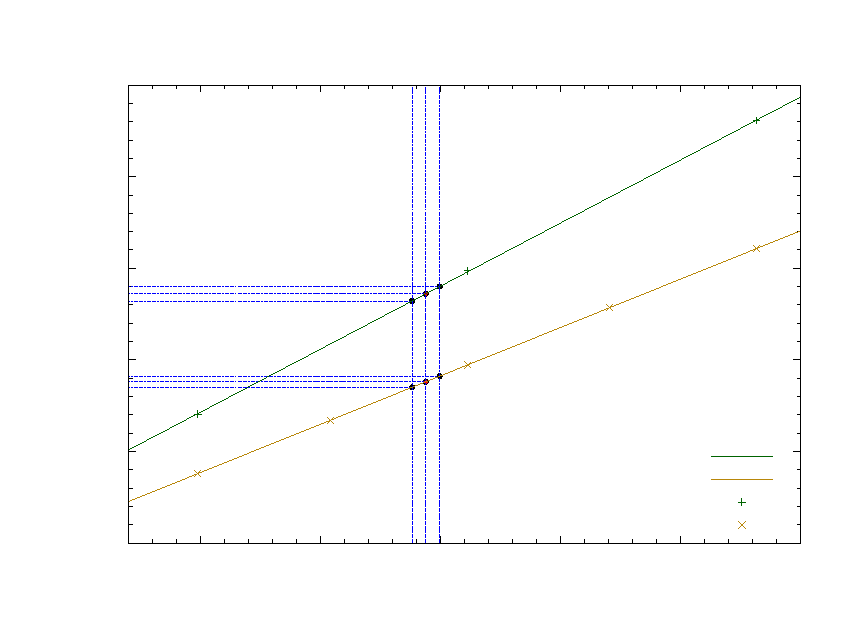
\includegraphics{tv5-plot}}%
    \gplfronttext
  \end{picture}%
\endgroup

			\caption{Zusammenhang zwischen $\ln\sbrace{\eta}$ und $\frac{1}{T}$}
			\label{fig:tvfive-plot}
		\end{figure}

		Abgelesen haben wir als Ergebnis die optimale Geraden:
		\begin{center}
			\begin{tabular}{llll}
				\toprule
				Ölsorte & Angepasste Kurve & Stoffkonstant & $\chi^2_\text{red}$ \\
				\midrule
				Rizinusöl & $\pbrace{\num{6878,02(4034)}}x - \pbrace{\num{23.4820(1378)}}$ & \SI{6880(40)}{\kelvin} & \num{4.41997e-05} \\
				Getriebeöl & $\pbrace{\num{5274.92(254)}}x - \pbrace{\num{18.5217(87)}}$ & \SI{5274.9(26)}{\kelvin} & \num{2.18987e-07} \\
				\bottomrule
			\end{tabular}
		\end{center}

		Da es explizit gefragt war, ist der Kehrwert $1/T$ und der dazugehörige Fehler $\Delta \pbrace{1/T}$ hier berechnet:
		\begin{align}
			\frac{1}{T} &= \frac{1}{\pbrace{\num{21.5} + \num{273.15}}~\si{\kelvin}} = \SI{3.39386e-3}{\per\kelvin} \sigfig{6} \\
			\Delta \pbrace{\frac{1}{T}} &= \frac{\Delta T}{T^2} = \frac{\SI{0.5}{\kelvin}}{\pbrace{\num{21.5} + \num{273.15}}^2~\si{\kelvin\squared}}=\SI{5.76e-6}{\per\kelvin} \sigfig{3}
		\end{align}
		Daraus folgt $1/T = \SI{3.394(6)e-3}{\per\kelvin}$

		Andere Rechnungen erfolgt in \gnuplot{} und wegen der Symmetrie der Fehler sind sie dann als $\pbrace{\max - \min}/2$ genommen. Mehr signifikante Ziffern als nötig werden in diesem Fall dargestellt, um mögliche Rundungsfehler zu vermeiden. Siehe Appendix \ref{appdx:tv5gnuplot} für die Rohausgabe aus \gnuplot{}.

		Abgelesen erhalten wir als Literaturwerte bei $T = \SI{21.5(5)}{\celsius}$:
		\begin{center}
			\begin{tabular}{lrrr}
				\toprule
				Ölsorte & $\mini{\eta_\text{~lit}}$ & $\maxi{\eta_\text{~lit}}$ & $\eta_\text{~lit}$ \\
				\midrule
				Rizinusöl & \SI{0,83651328}{\pascal\second} & \SI{0,90548028}{\pascal\second} & \SI{0,87(4)}{\pascal\second} \\
				Getriebeöl & \SI{0,52221602}{\pascal\second} & \SI{0,55492858}{\pascal\second} & \SI{0,538(17)}{\pascal\second} \\
				\bottomrule
			\end{tabular}
		\end{center}

		Im Vergleich zu unserem empirischen Wert $\eta_\text{~exp} = \SI{0.495(5)}{\pascal\second}$ ist es dann höchstwahrschein\-lich, dass Getriebeöl im Experiment verwendet wurden. Es ist aber offentsichlich, dass die zwei Werte unterscheiden sich signifikant voneinander.

		Dieser Unterchied kann vermütlich darauf zurückgeführt werden, dass es bei der kleinen Kugel im weiten Rohr immer noch verwirbelungen bzw. Reibungseffekte gibt, die im Rechnungen nicht berücksichtigt wurden. Das kann beispielweise entstehen, wenn die Kugeln nicht gut gesaubert waren. Die Fallzeit der kleinen Kugel war auch etwas ungenau und es könnte sein, dass die Ungenauigkeit der Zeitmessung unterschätzt war. Da die Temperatur und Dichte des Öls nicht vom benutzten Ölrohr gelesen wurden, könnte es auch sein, dass die abgelesene Werte nicht die echte Parameter beim Experiment sind. 

\resnum
\newpage
\appendix
\section{\gnuplot{} Quellcode zur Auswertung von Teilversuch 2}
    \label{appdx:gnuplotTV2}
    
    \gnuplot{} Code für Abbildung \ref{fig:stoppuhr}
    {  
        % % Surpress "errors" in minted
        % https://tex.stackexchange.com/a/289068
        \renewcommand{\fcolorbox}[4][]{#4}
        \begin{minted}[linenos,breaklines,autogobble,frame=leftline,framesep=10pt]{gnuplot}
            set term epscairo font "Linux Libertine, 14" size 5in, 4in
            set output "maxwell.eps"
            set decimalsign locale 'de_DE.UTF-8'

            set title "Zusammenhang zwischen Schwingungsdauer und maximaler Höhe\n(Nach Augenmaß)"
            set xlabel "Quadrate der Schwingungsdauer (s^2)"
            set ylabel "Höhe (mm)"
            set key left top

            f(x) = m*x + c

            # (x, y, xdelta, ydelta)
            fit f(x) "maxwell.dat" u ($2**2):1:($2*2*(0.5)):(5) xyerrors via m,c

            set yrange [200:900]
            set xrange [15:125]

            t = gprintf("%.3f", m)."x + ".gprintf("%.3f", c)
            plot f(x) title t, "maxwell.dat" u ($2**2):1:($2*2*(0.5)):(5) with xyerrorbars pointtype 0 title "maxwell.dat"
        \end{minted}
    }
    mit \texttt{maxwell.dat}:
    \begin{minted}[linenos,breaklines,autogobble,frame=leftline,framesep=10pt]{text}
        # Höhe  T
        775 10,57
        715 9,53
        665 10,1
        647 8,92
        583 8,89
        550 8,76
        515 7,79
        485 7,59
        465 7,92
        430 7,4
        405 7,03
        387 6,52
        365 6,41
        345 6,55
        330 5,64
        315 6,07
        300 5,3
        296 5,48
        275 5,04
        260 4,69
        250 4,76
    \end{minted}

\section{\texttt{Python} Code zur Bestimmung des Fehlers $\Delta R_J$}
    \label{appdx:pythonTV2}

    \begin{minted}[linenos,breaklines,autogobble,frame=leftline,framesep=10pt]{python}
        #!/usr/bin/env python3

        import numpy as np

        def rj(l1, l2, l3, l4, r1, r2, r3, r4, r5):
            return np.sqrt((0.5)*((l1*r1**4 + l2*(r2**4-r1**4) + l3*(r3**4-r2**4+r5**4-r4**4) + l4*(r4**4-r3**4))/(l1*r1**2 + l2*(r2**2-r1**2) + l3*(r3**2-r2**2+r5**2-r4**2) + l4*(r4**2-r3**2))))

        def parameterize(*args):
            return args

        maxWert = 0
        minWert = 100
        step = 0.01

        for i1 in range(-5,6,2):
            for i2 in range(-5,6,2):
                for i3 in range(-5,6,2):
                    for i4 in range(-5,6,2):
                        for i5 in range(-5,6,2):
                            for i6 in range(-5,6,2):
                                for i7 in range(-5,6,2):
                                    for i8 in range(-5,6,2):
                                        for i9 in range(-5,6,2):
                                            currWert = rj(141.675 + i1*step, 63.275 + i2*step, 6.575 + i3*step, 2.025 + i4*step, 4.05 + i5*step, 6.525 + i6*step, 10.25 + i7*step, 67.85 + i8*step, 87.05 + i9*step)
                                            params = parameterize(141.675 + i1*step, 63.275 + i2*step, 6.575 + i3*step, 2.025 + i4*step, 4.05 + i5*step, 6.525 + i6*step, 10.25 + i7*step, 67.85 + i8*step, 87.05 + i9*step)

                                            if currWert > maxWert:
                                                maxWert = currWert
                                                maxParams = params
                                            if currWert < minWert:
                                                minWert = currWert
                                                minParams = params

        print("Max Value\t", maxWert)
        print("Max Params\t", maxParams)
        print("Min Value\t", minWert)
        print("Min Params\t", minParams)
    \end{minted}

    Rohausgabe:
    \begin{minted}[linenos,breaklines,autogobble,frame=leftline,framesep=10pt]{text}
        Max Value    65.50959631684215
        Max Params   (141.625, 63.225, 6.625, 1.9749999999999999, 4.0, 6.4750000000000005, 10.2, 67.8, 87.1)
        Min Value    64.94975893345266
        Min Params   (141.72500000000002, 63.324999999999996, 6.525, 2.0749999999999997, 4.1, 6.575, 10.3, 67.89999999999999, 87.0)
    \end{minted}
    Wertetabelle zur Vergleichung:
    \begin{multicols}{2}
        \begin{center}
            \begin{tabular}{lrl}
                \toprule
                Variable & Wert \\
                \midrule
                $L_1$ & \SI{141,675(50)}{\milli\meter} \\
                $L_2$ & \SI{63,275(50)}{\milli\meter} \\
                $L_3$ & \SI{6.575(50)}{\milli\meter} \\
                $L_4$ & \SI{2.025(50)}{\milli\meter} \\
                \bottomrule
            \end{tabular}
        \end{center}
        \begin{center}
            \begin{tabular}{lrl}
                \toprule
                Variable & Wert \\
                \midrule
                $R_1$ & \SI{4,05(5)}{\milli\meter} \\
                $R_2$ & \SI{6.525(50)}{\milli\meter} \\
                $R_3$ & \SI{10.25(5)}{\milli\meter} \\
                $R_4$ & \SI{67.85(5)}{\milli\meter} \\
                $R_5$ & \SI{87.05(5)}{\milli\meter} \\
                \bottomrule
            \end{tabular}
        \end{center}
    \end{multicols}

\section{\texttt{Python} Code zur Bestimmung des Wertes und Fehlers von $J_d$ im Teilversuch 3}
    \label{appdx:pythonJd}

    \begin{minted}[linenos,breaklines,autogobble,frame=leftline,framesep=10pt]{python}
        #!/usr/bin/env python3
        import numpy as np

        # x. y, z
        L      = np.array([5.115e-2, 7.315e-2, 10.250e-2])
        deltaL = 0.005e-2
        J      = np.array([3.95523e-3, 3.29182e-3, 2.04429e-3])
        deltaJ = np.array([3.177e-5, 4.851e-5, 5.736e-5])

        r = np.dot(L, L)

        vecL2 = np.multiply(L, L)
        vec1 = np.multiply(J, r - vecL2)

        def Jd():
            return (1/r)*(np.dot(J, vecL2))

        def deltaJd():
            return (1/r)*np.sqrt(((4*deltaL**2)/(r**2))*(np.dot(vec1, L))**2 + (np.dot(vecL2, deltaJ))**2)

        print("J_d Wert\t", Jd())
        print("Delta J_d\t", deltaJd())
    \end{minted}

    Rohausgabe:
    \begin{minted}[linenos,breaklines,autogobble,frame=leftline,framesep=10pt]{text}
        J_d Wert     0.0026762804092092477
        Delta J_d    5.122652638090954e-05
    \end{minted}
\end{document}
